\chapter{Value-based RL model}
\label{chap:SimpRL}
The models presented in \hyperref[chap:RLModel]{~Chapter \ref*{chap:RLModel}} assume the lick to be a functional action, which is reasonable in our case because the task presented is conditioned to the animal performing three licks before reward. However, it is possible to build a simplified value-based version of the hybrid Rescorla-Wagner model, without explicitly considering licks as actions.\\Thus the expected reward values are expressed as follows:
\begin{equation}
V_s(t+1)=V_s(t)+k\cdot\alpha(t)\cdot\delta  \hspace{0.3cm} with \hspace{0.3cm}\delta(t)=r(t)-V_s(t)
\label{VValues}
\end{equation}
where V is now a $
T\times 2$ vector, with $t$ the trials index and $T$ the number of trials. $\delta$ is the prediction error. Importantly V values are still modulated according to the time dependent component $\alpha(t)$, related to the uncertainty about the possible outcome.
\begin{equation}
    \alpha(t)=(1-\eta)\cdot\alpha(t-1)+\eta\cdot\abs{\delta(t)},\hspace{0.3cm} \eta\in[0,1]
\end{equation}
%The need to introduce a time dependent learning rate was emphasized first in works as \cite{Daw} and \cite{Funamizu}.
In figure \ref{fig:PavRL_ex} is shown an example of, from the top to the bottom, the performance, the reward expectation values $V$, the uncertainty $\alpha$ and the reward prediction error $\delta$.
\begin{figure}
    \centering
    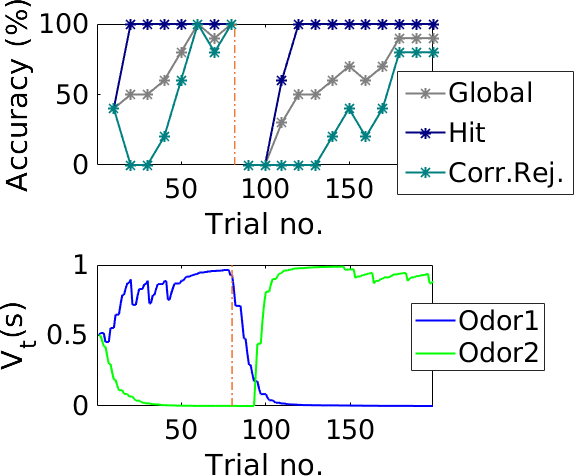
\includegraphics[scale=0.7]{figures/PavPerfV.png}
    
    \vspace{0.5cm}
    
    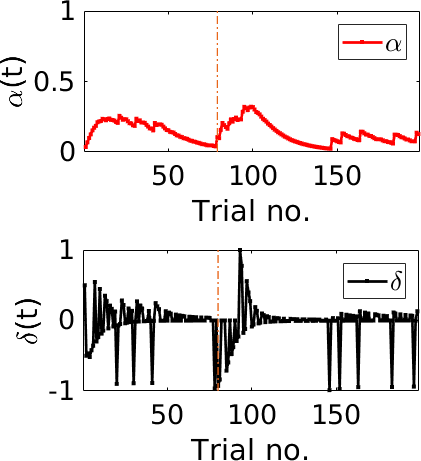
\includegraphics[scale=0.7]{figures/PavAlphaDelta.png}
    \caption{From the top to the bottom, the animal performance, the reward expectation values $V$, the uncertainty $\alpha$ and the reward prediction error $\delta$.}
    \label{fig:PavRL_ex}
\end{figure}
I tested whether SPN-DAN pairs encode reward prediction error signals as done in \hyperref[sec:Regression]{~Chapter \ref*{sec:Regression}}. 
The hypothesis was tested regressing out $\alpha$ and $\delta$ in two distinct Poisson regression models, where the observations are the SPN-DAN pairs activity. The processes were modeled as follows:
\begin{equation*}
    \log(\mu_t)=\beta_0+\beta\cdot\alpha(t-1)
\end{equation*}
and 
\begin{equation*}
    \log(\mu_t)=\beta_0+\beta\cdot\delta(t)
\end{equation*}
Coefficients $\beta$ were transformed as shown in equations \ref{eq:BetaPerc} and \ref{eq:BetaPlot} to be interpreted as a change in percentage of assembly-activity. For detailed discussion on Poisson regression coefficients and their interpretation see \hyperref[sec:Regression]{~Chapter \ref*{sec:Regression}}.\\
In figure \ref{fig:RL_alphadelta} I show on the left side box plots of standardized regression coefficients $\beta^*$, on the right side empirical cumulative distribution function of $\beta^*$.\\
\begin{figure}
   \centering
    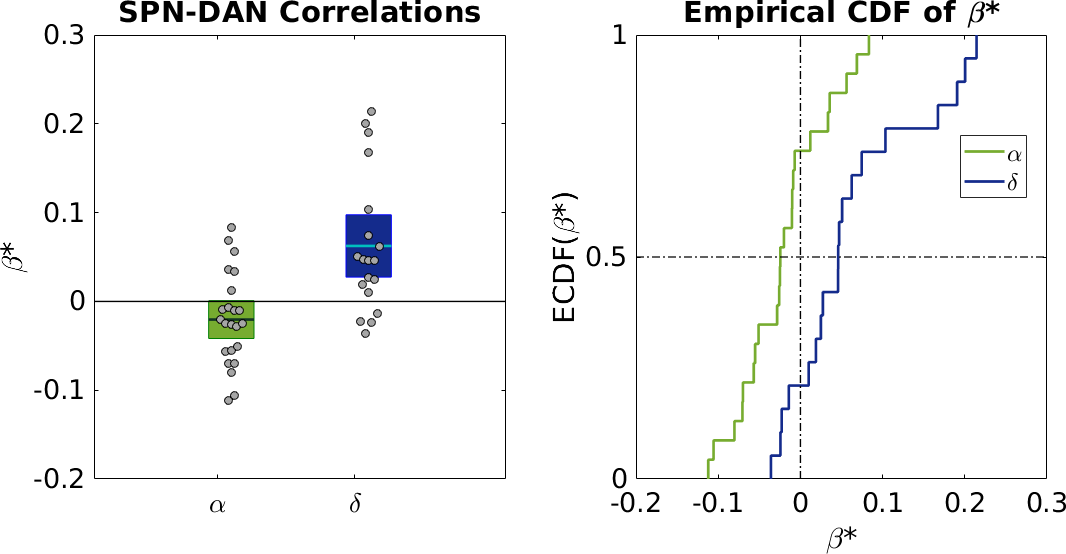
\includegraphics[scale=0.45]{figures/AlphaAndDeltaPavSPN3.png}
    \caption{$\alpha$ and $\delta$ were regressed out in two separated Poisson regression models with the SPN-DAN pairs activity. \textbf{Left:} box plot of standardized regression coefficients $\beta^*$. \textbf{Right:} empirical cumulative distribution function of $\beta^*$}
    \label{fig:RL_alphadelta}
\end{figure}
The regressions of $\alpha$ and $\delta$ show, in line with what has been presented in \hyperref[sec:Regression]{~session \ref*{sec:Regression}} (see figure \ref{fig:AlphaDeltaReg}), that SPN-DAN pairs anti-correlate with the uncertainty $\alpha$ whilst correlate with $\delta$, supporting the hypothesis that those assembly-pairs specifically encode the reward prediction error. However the anti-correlation effect with $\alpha$ is much less evident using hybrid Rescorla-Wagner without licks as functional actions, than using the learning-forgetting model proposed in \hyperref[chap:RLModel]{~Chapter \ref*{chap:RLModel}}. The importance to consider he lick as functional action is implicit in the structure of the task, in which the $"$no-lick$"$ is part of the learning as well as the $"$lick$"$.\\In the near future I plan to set up a formal model comparison method which includes all models presented in \hyperref[chap:RLModel]{~Chapter \ref*{chap:RLModel}} and in \hyperref[chap:SimpRL]{~Appendix \ref*{chap:SimpRL}}. To this aim I could apply a the Bayesian model selection (BMS), already used for similar problems, which consists of a hierarchical Bayesian framework which, evaluates which model better represents the animals$'$ behavior through estimation of the posterior probabilities for the respective models given the observed animals$'$ actually behavioral choices (\cite{Koppe}), or the integrated Bayesian information criterion (iBIC), used in works in which both nested and not nested models were compared (\cite{Dayan}).